\documentclass[12pt,letterpaper]{article}
\usepackage[margin=1in]{geometry}
\usepackage[intlimits]{amsmath}
\usepackage{graphicx}
\usepackage{fancybox}
\usepackage{ifthen}
\usepackage{url}
\usepackage{lscape,afterpage}
\usepackage{xspace}
\usepackage{epstopdf} 
\usepackage{subcaption}
\graphicspath{{Figures/}}
\begin{document}
\title{Technical Note: $^{11}$C Spallation Production Measurement}
\author{Hasung Song}
\maketitle
\begin{abstract}
	This technical note describes the $^{11}$C measurement in KLZ and how the rate is extracted.
\end{abstract}

\subsection*{Spallation Event Selection}
\begin{itemize}
	\item Standard FBE muon selection cuts
	\item Standard MoGURA neutron selection cuts
	\item Neutron Shower Cuts ($N_n=1$)
	\item $0\nu\beta\beta$ selection cuts, except for spallation-related cuts
	\item XeLS $^{11}$C Candidate cuts
	\begin{itemize}
		\item Energy Range  : 1.0-1.6 MeV
		\item Radius : 0-160 cm
		\item dT : 100-18,000 s (5 hours)
	\end{itemize}
	\item KamLS $^{11}$C Candidate cuts
	\begin{itemize}
		\item Energy Range  : 1.4-2.4 MeV
		\item Radius : 220-350 cm
		\item dT : 100-18,000 s (5 hours)
	\end{itemize}
	\item $dR$ Cut : $<80$ cm
\end{itemize}

\subsection*{Fit to $dT$}
dT of muon-event pairs where the neutron shower contained 1 observed neutron is shown in Figure \ref{fig:dT_fits}.
\begin{figure}[ht]
	\centering
	\subcaptionbox{XeLS\label{fig:dT_XeLS}}[0.45\textwidth]{
		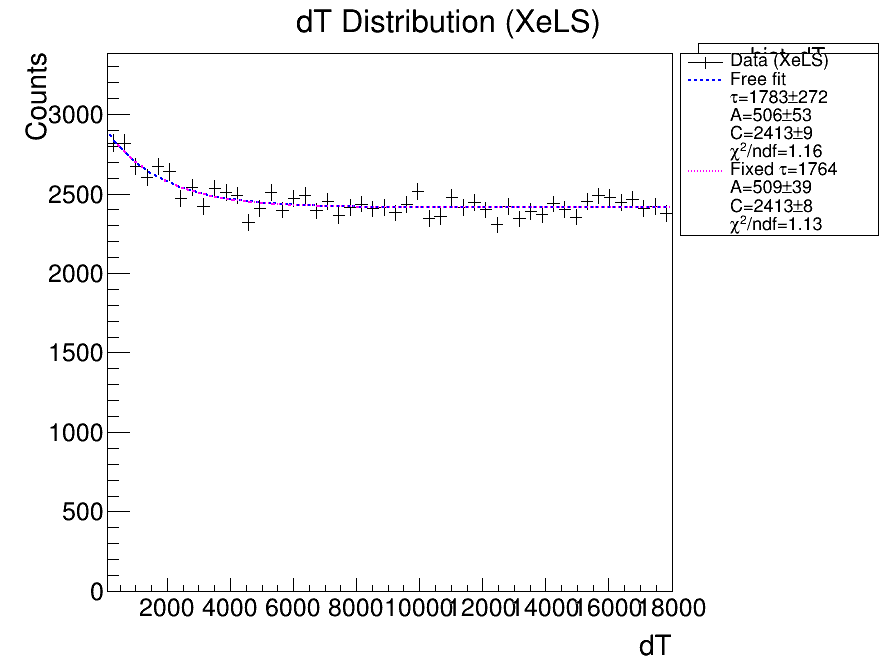
\includegraphics[width=0.45\textwidth]{dT_distribution_allcuts_XeLS.png}}
	\hfill
	\subcaptionbox{KamLS\label{fig:dT_KamLS}}[0.45\textwidth]{
		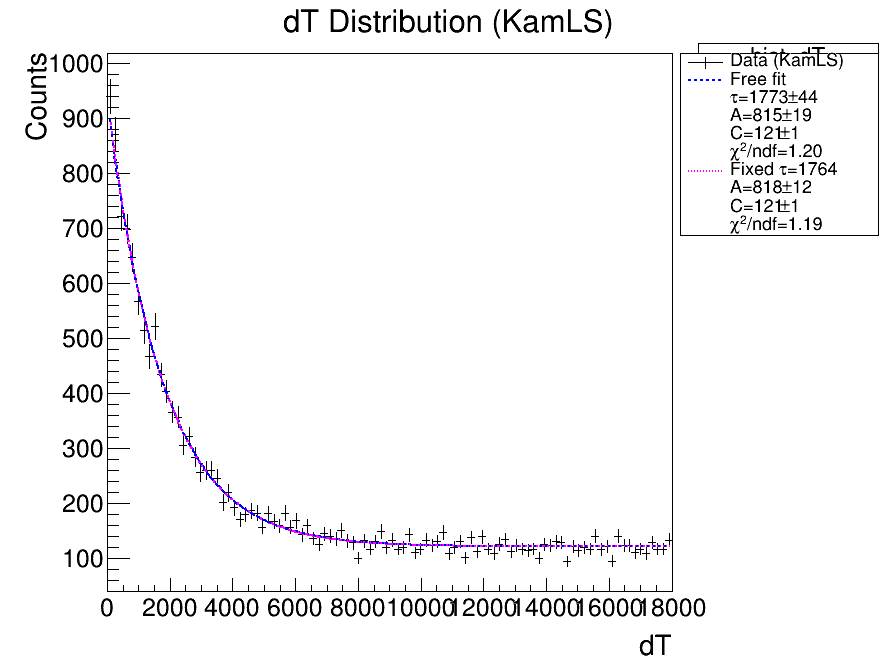
\includegraphics[width=0.45\textwidth]{dT_distribution_allcuts_KamLS.png}}
	\caption{dT of muon-event pairs where the neutron shower contained 1 observed neutron.}
	\label{fig:dT_fits}
\end{figure}

\subsection*{Rate Calculation}
The calculation of expected number of detected, selected, and correlated $^{11}$C-$\mu$ pairs. Not trying to calculate the expected number of background "accidentally correlated muon-event pairs", only the true $^{11}$C-$\mu$ pairs.
\begin{equation}
	% I_{C11} = Y_{C11}\times E_{FBE} \times (1-dt_{MoG}) \times P_n(1|^{11}C_{spall}) \times \epsilon_{dR} \times \epsilon_{dT} \times \epsilon_{FV} \times \epsilon_{E}
	I_{C11} = Y_{C11}\times E_{FBE} \times (1-dt_{MoG}) \times \epsilon_{dR} \times \epsilon_{dT} \times \epsilon_{FV} \times \epsilon_{E}
\end{equation}
\begin{itemize}
	\item $I_{C11}$: Integral of the exponential component of the fit, "Observed $\mu-^{11}$C pairs"  $[events]$
	\begin{equation}
		I_{C11} = A_{C11}\cdot \tau\cdot \frac{e^{\frac{-100}{\tau}}-e^{\frac{-18000}{\tau}}}{(18000-100)/50}
	\end{equation}
	\begin{itemize}
		% \item \textbf{XeLS  : 2,370 events}
		\item \textbf{XeLS  : 10,153 events}
		\item \textbf{KamLS : 3,794 events}
		\item Used the fit with fixed $^{11}C$ lifetime
		\item $(18000-100)/50 $s is the dT histogram bin spacing
	\end{itemize}
	\item $Y_{C11}$: \textbf{Final Result} Production rate of $^{11}$C in KamLS, XeLS $[events/kton\cdot days]$
	\item $E_{FBE}$: Exposure, Livetime : $[kton\cdot days]$
	\begin{itemize}
		% \item \textbf{XeLS : 11.96 kton-days} 
		\item \textbf{XeLS : 16.36 kton-days} 
		\item \textbf{KamLS : 130.68 kton-days}
		\item Volume of the target region, density, Livetime
		\item LiveTime excludes the first 5 hours of each FBE run
	\end{itemize}
	\item $dt_{MoG}$: MoGURA Deadtime Fraction: [unitless]
	\begin{itemize}
		\item \textbf{1.88\%}
		\item simply scale up based on the deadtime since muons that occur during deadtime will not be able to create accurate pairs.
		\item Go through the FBE and MoGURA runs and check for overlap.
	\end{itemize}
	% \item $P_n(1|^{11}C_{spall})$: Neutron Production : How many muons that create $^{11}$C create exactly 1 \textbf{observed} neutron [unitless]
	% \begin{itemize}
	% 	\item \textbf{XeLS : 27.9\%}
	% 	\item \textbf{KamLS : 28\%}
	% 	\item Muons that create $^{11}$C, in the target volumes (KamLS, XeLS), and create $1+$ neutrons, some fraction of those have only one detected (Toy MC calculation using Neutron Tagging Efficiency and FLUKA simulated neutron yield)
	% 	\item Used Kelly's new FLUKA simulations with a wider FV and realistic scintillator volume geometry
	% 	\item \verb|/userdata/work/kweerman/FLUKA/FLUKA-muon-spallation/root/XeLS_Minus_d500|
	% \end{itemize}
	\item $\epsilon_{dR}$: $dR<80$ cm cut efficiency (from FLUKA tuned with $^{11}$C), for each data period [unitless]
	\begin{itemize}
		\item \textbf{XeLS : 57\%}
		\item \textbf{KamLS : 56.4\%}
		\item Also from Kelly's new FLUKA simulation
	\end{itemize}
	\item $\epsilon_{dT}$: dT $>100$s cut efficiency (from known $^{11}$C half-life) [unitless]
	\begin{itemize}
		\item \textbf{94.5\%}
		\item Simply integrate the exponential decay distribution between 100-18,000 s
	\end{itemize}
	\item $\epsilon_{FV-E}$: Fiducial Volume \& Energy Cut Efficiency (KLG4Sim) [unitless]
	\begin{itemize}
		\item \textbf{XeLS : 79.7\%}
		\item \textbf{KamLS : 40.5\%}
		\item Calculate the efficiency from the energy and radius cuts described in the first section.
	\end{itemize}
\end{itemize}
Simply solve for $Y_{C11}$:
\begin{equation}
	% Y_{C11} = \frac{I_{C11}}{E_{FBE} \times (1-dt_{MoG}) \times P_n(1|^{11}C_{spall}) \times \epsilon_{dR} \times \epsilon_{dT} \times \epsilon_{FV} \times \epsilon_{E}}
	Y_{C11} = \frac{I_{C11}}{E_{FBE} \times (1-dt_{MoG}) \times \epsilon_{dR} \times \epsilon_{dT} \times \epsilon_{FV-E}}
\end{equation}

\subsection*{Systematic Errors}
\begin{itemize}
	% \item $A_{C11}$, exponential amplitude, fit uncertainty : $A_{C11}=509\pm39$, $\frac{39}{504}=7.7\%$
	\item $A_{C11}$, exponential amplitude, fit uncertainty : $A_{C11}=2,181\pm87$, $\frac{87}{2,181}=4.0\%$
	\item Exposure Uncertainty, from $0\nu$ analysis uncertainty $\sim 4\%$
	\begin{itemize}
		\item 4\% uncertainty stated for uncertainty in xenon exposure, mainly driven by FV uncertainty, similar for Carbon?
	\end{itemize}
	\item Neutron Tagging Efficiency Error: $74.5\%\pm0.4\%$
	\item FLUKA simulation Systematic : dR Cut, Neutron Production
	\item FLUKA simulation Statistical (insignificant)
	\item Energy Scale Uncertainty : (use 1 sigma of kB, R contour)
\end{itemize}

\subsection*{Results}
\begin{itemize}
	% \item \textbf{XeLS} : $1,690\ events/day/kton$
	\item \textbf{XeLS} : $1,470\ events/day/kton$
	\item \textbf{KamLS} : $669\ events/day/kton$
\end{itemize}

Previous results from KamLAND: $1,106\pm178$ events/day/kton 2009 spallation paper, $973\pm10$ events/day/kton from $^{7}Be$ solar neutrino measurement.

There is a large discrepancy between my results and the previous measurements. Also the trend is inconsistent, XeLS rate is too high, KamLS rate is too low.
\subsection*{Possible Errors}
\begin{itemize}
	\item different livetime for different volume regions?
	\item Different event selection efficiency for different volume regions? Currently using the standard selection for $0\nu\beta\beta$ analysis.
\end{itemize}


\end{document}